% Extracao de entidades (NER) com frases do corpus do prototipo (rasa\data\nlu.yml).
% Gera fig_ner_exemplo.png.
\documentclass[border=8pt]{standalone}
\usepackage[utf8]{inputenc}
\usepackage[T1]{fontenc}
\usepackage{tikz}
\usetikzlibrary{positioning,arrows.meta,calc,fit,backgrounds}
\renewcommand{\familydefault}{\sfdefault}
\tikzset{
  caixa/.style={rectangle, rounded corners=4pt, draw, fill=white, align=left, inner sep=6pt},
  ent/.style={rectangle, rounded corners=2pt, fill=blue!12, inner sep=1.5pt},
  seta/.style={-{Latex[length=3mm]}, line width=1.4pt},
  titulo/.style={font=\bfseries},
}
\newcommand{\e}[1]{\tikz[baseline=(x.base)]\node[ent] (x) {#1};}
\begin{document}
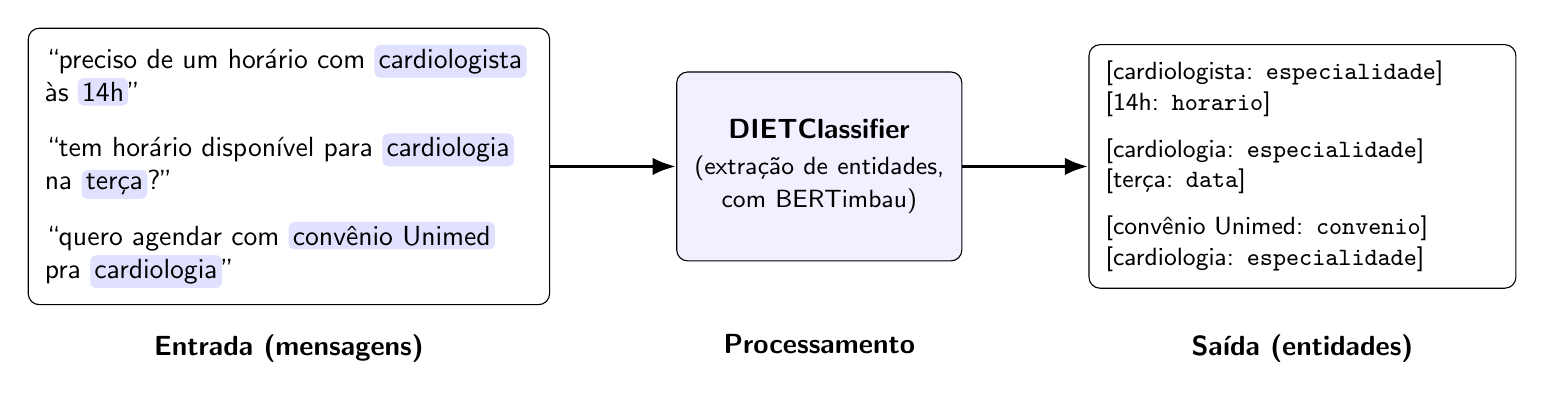
\begin{tikzpicture}
\node[caixa, text width=6.2cm] (ent) {%
  ``preciso de um horário com \e{cardiologista} às \e{14h}''\\[8pt]
  ``tem horário disponível para \e{cardiologia} na \e{terça}?''\\[8pt]
  ``quero agendar com \e{convênio Unimed} pra \e{cardiologia}''};
\node[caixa, align=center, text width=3.2cm, right=1.6cm of ent, fill=blue!6, minimum height=2.4cm]
  (proc) {\textbf{DIETClassifier}\\[2pt]\small (extração de entidades,\\com BERTimbau)};
\node[caixa, text width=5.0cm, right=1.6cm of proc, font=\small] (sai) {%
  [cardiologista: \texttt{especialidade}]\\{}[14h: \texttt{horario}]\\[6pt]
  {}[cardiologia: \texttt{especialidade}]\\{}[terça: \texttt{data}]\\[6pt]
  {}[convênio Unimed: \texttt{convenio}]\\{}[cardiologia: \texttt{especialidade}]};
\draw[seta] (ent.east) -- (proc.west);
\draw[seta] (proc.east) -- (sai.west);
\node[titulo, below=0.25cm of ent] {Entrada (mensagens)};
\node[titulo, below=0.25cm of proc |- ent.south] {Processamento};
\node[titulo, below=0.25cm of sai |- ent.south] {Saída (entidades)};
\end{tikzpicture}
\end{document}
